% Last updated: 2023/02/19 22:14:03
\documentclass[12pt,a4j]{jreport}
\usepackage{klthesis}
\usepackage{amsmath}
\usepackage{listings, jlisting}

\lstset{
basicstyle={\ttfamily},
language=Python,
identifierstyle={\small},
keywordstyle={\small\bfseries},
ndkeywordstyle={\small},
stringstyle={\small\ttfamily},
frame={tb},
breaklines=true,
columns=[l]{fullflexible},
numbers=left,
xrightmargin=0zw,
xleftmargin=3zw,
numberstyle={\scriptsize},
stepnumber=1,
numbersep=1zw,
lineskip=-0.5ex
}

\begin{document}

\type{B} %卒論はB,修論はM
\author{須崎 良祐}
\id{27020729} %学籍番号
\fyear{2024} %修了・卒業年度(修了・卒業式が2024年3月なら2023年度)
\title{飲食店推薦のための\\機械学習アルゴリズムの比較}
\abstract{
  本研究は,飲食店の推薦において,決定木,ロジスティック回帰,k-NNのうち,どの機械学習アルゴリズムが適しているかを明確化することを目的としている. 
  
  本研究では,飲食店に関するデータを入力変数に変換し,飲食店に対する評価を目的変数に変換し,決定木,ロジスティック回帰,k-NNの3つのモデルで性能の比較を行った.
  
  実験は,十分な飲食店情報と評価データが利用可能な場合に行われた.
  また,それらの情報を減らした際の精度の推移も確認した.
  その結果,情報が豊富な場合には決定木が最良の結果を示した.

  この研究は,機械学習を用いた推薦アルゴリズムの開発において,使用するアルゴリズムの選択が学習量データの量に依存することを示している.
  それにより,学習用データの量が少ない場合と多い場合に,3つのアルゴリズムから,どのアルゴリズムを選択すればいいかといった考察を提供している.
}

\maketitle

% 1章

\chapter{はじめに}

飲食店推薦システムは,ユーザーの過去の行動や好みに基づき,自動的に関連する飲食店を提案する技術である.
このようなシステムは,ユーザーがまだ発見していない新しい飲食店を提案することで,個人化された食体験を提供する.

これは,ぐるなびや食べログなどの検索システムとは明確に異なる.
これらの検索システムでは,ユーザーは特定の検索条件を入力し,システムはそれに最も適した飲食店情報を提供する.
一方で,推薦システムでは,ユーザーの飲食店に対する過去の評価を分析し,ユーザー自身が未知である可能性のある新しい飲食店を提案する.
つまり,推薦は自動的にユーザーに対して飲食店情報を提供し,検索はユーザー自身が飲食店情報を見つけ出さなければならないのである.

ユーザーの手間がかからない点や新しい未知の飲食店を発見できる可能性が高い点は,飲食店推薦システムの大きな価値となっている.
飲食店の推薦は,爆大な飲食店情報から,好みに合った飲食店の情報を提供する.

近年では推薦システムの研究は盛んに行われているが,本研究では2つの研究を関連研究として取り上げる.
1つ目は,決定木を用いたユーザー群に対しての飲食店推薦システムの研究\cite{a}であるが,ユーザー群に対しての推薦システムになっているため, 個人の好みに着目した推薦をすることができない.
2つ目は,ユーザー個人の飲食店に対する評価によって価格帯とジャンルそれぞれに対する重みが変動し,そのユーザーの好みに沿った飲食店を提示できる推薦システムの研究\cite{b}であるが,推薦に用いる飲食店情報として,価格帯とジャンルしか扱っていない.
また,決定木を用いたユーザー個人で利用できる音楽推薦システムの研究\cite{c}もあり,決定木と他の機械学習アルゴリズムを比較して,決定木の有効性を示している.
しかし,飲食店推薦の文脈で,どの機械学習アルゴリズムが有効であるか明確でない.

そこで,本研究では,飲食店推薦に,代表的な機械学習アルゴリズム(決定木,ロジスティック回帰,k-NN)のうち,どのアルゴリズムを使えば良いかを明確化する.

評価では,飲食店情報とそれに対するユーザーの評価を用いて, 各機械学習アルゴリズムで10フォールド交差検証を行い, その性能を示す.
また,学習用データを増やした際の精度の推移を示す.

本論文の構成は以下の通りである.
第2章では,関連研究,及び本研究の目的について述べる.
第3章では,本研究で比較する機械学習アルゴリズムの詳細について述べる.
第4章では,結果その考察を述べる.
第5章では,本研究のまとめと今後の課題について述べる.

% 2章

\chapter{推薦システム}

\section{推薦システム}

推薦システム\cite{d}は,ユーザーの行動パターンに基づいて,商品,サービス,情報といったアイテムを自動的に提案するシステムである.
このシステムの重要性は,インターネットの発展とともに急速に増しており, 背景として情報過多の問題がある.
現代のデジタル社会で,ユーザーが直面する情報の量が爆発的に増加し,関連性の高い,または興味を引くコンテンツを効率的に見つけることが困難になっているためである.

推薦システムは,この情報の海から有用な情報を引き出し,個々のユーザーにカスタマイズされた推薦を行うことで,情報選択のプロセスを簡素化し,ユーザー体験を向上させる.

推薦システムの開発は,ユーザーのニーズを理解し,パーソナライズされたサービスを提供することに重点を置いている.
これにより,ユーザー満足度を高め,ビジネスにおいては顧客の関与を深め,売上向上に寄与することが期待される.

推薦システムにおいて広く使用される2つの主要な手法は,以下の通りである.\\\\
\textbf{内容ベースフィルタリング}\\
内容ベースフィルタリングは,ユーザーのアイテムに対する過去の評価を分析し,アイテムの各特徴とユーザーの評価の関係をモデル化し,そのモデルを用いて新たなアイテムを推薦する手法である.
つまり,アイテムの特徴に着目している.

表\ref{rate_content_table}において,ユーザーAに飲食店を推薦する場合を考える. 
ここでは,「無し」を0,「有り」を1という特徴量にする.
内容ベースフィルタリングの場合,ユーザーAが高評価した飲食店と似た特徴を持つ飲食店を推薦する.
ユーザーAは,飲食店Aに高評価した場合,飲食店Aと最も類似度が高い飲食店BをユーザーAに推薦する.\\\\\\
\textbf{協調フィルタリング}\\
協調フィルタリングは,多くのユーザーのアイテムに対する評価を分析し,似た評価パターンを持つユーザーを見つけ出し,新たなアイテムを推薦する手法である.

表\ref{rate_coll_table}において,ユーザーAに飲食店を推薦する場合を考える.
ここでは,「行きたくない」を0,「行きたい」を1という評価値にする.
協調フィルタリングの場合,ユーザーAと似た評価パターンを持つユーザーを元に推薦を行う.
ユーザーAは,ユーザーDと最も類似度が高い評価パターンを持つため,ユーザーDが「行きたい」と評価した飲食店DをユーザーAに推薦する.\\

つまり,内容ベースフィルタリングはユーザーの評価とアイテムの特徴の関係を用いる推薦手法であり,協調フィルタリングは他ユーザー,あるいは他アイテムの評価パターンを用いる推薦手法である.

本研究では,内容ベースフィルタリングを用いた推薦に焦点を当てている.\\

\begin{table}[htbp]
  \begin{center}
    \begin{tabular}{|l|r|r|r|r|}\hline
      \textbf{特徴/飲食店} & 飲食店A & 飲食店B & 飲食店C & 飲食店D \\ \hline
      喫煙席の有無       & 0        & 0        & 1        & 1 \\ \hline
      駐車場の有無       & 1        & 1        & 0        & 0 \\ \hline
      Wi-Fiの有無       & 1        & 0        & 0        & 0 \\ \hline
      個室の有無         & 1        & 1        & 0        & 1 \\ \hline
    \end{tabular}
  \end{center}
  \caption{飲食店の特徴量}
  \label{rate_content_table}
\end{table}

\begin{table}[htbp]
  \begin{center}
    \begin{tabular}{|l|r|r|r|r|}\hline
      \textbf{ユーザー/飲食店} & 飲食店A & 飲食店B & 飲食店C & 飲食店D \\ \hline
      ユーザーA       & 1        & 1        & -        & - \\ \hline
      ユーザーB       & 1        & 0        & 1        & 1 \\ \hline
      ユーザーC       & 0        & 1        & 1        & 0 \\ \hline
      ユーザーD       & 1        & 1        & 0        & 1 \\ \hline
    \end{tabular}
  \end{center}
  \caption{ユーザーの飲食店に対する評価値}
  \label{rate_coll_table}
\end{table}

\section{推薦システムに関する研究}
\subsection{決定木を用いたユーザー群に対しての飲食店推薦\cite{a}}
この研究では,決定木を用いて,飲食店を低価格帯,中価格帯,高価格帯カテゴリに分類し,ユーザーを低予算,中予算,高予算カテゴリに分類し,各カテゴリがマッチする飲食店をユーザーに推薦するシステムの開発を行っている.
この研究で用いたデータセットには表\ref{master_table}のような95件の飲食店情報と,135人の顧客情報と顧客のいくつかの飲食店に対する評価情報が含まれいる.
これらの情報を使って,ユーザーを各予算カテゴリ,飲食店を各価格帯カテゴリに分類する決定木を構築している.
システムの構成として,顧客情報を入力し,それに基づいて飲食店情報が出力される.

しかし,この研究で開発しているシステムは,他人の顧客情報と飲食店に対する評価を使った推薦システムになっているため,個人の好みに着目した推薦を行うことができないという課題を抱えている.\\

\begin{table}[htbp]
  \begin{center}
    \begin{tabular}{|l|l|}\hline
      \textbf{顧客情報} & \textbf{飲食店情報} \\ \hline
      ユーザーID & 飲食店ID \\
      緯度 & 料理 \\
      経度 & 支払い方法 \\
      喫煙者かどうか & 駐車場 \\
      飲酒レベル & 平日の営業時間 \\
      服装の好み & 土曜の営業時間 \\
      雰囲気 & 日曜の営業時間 \\
      交通手段 & 緯度 \\
      婚姻状況 & 経度 \\
      子供の有無 & 名前 \\
      生年 & 提供アルコール \\
      興味・関心 & 喫煙エリア \\
      性格 & 服装コード \\
      宗教 & アクセシビリティ \\
      活動レベル & 価格帯 \\
      色 & 雰囲気 \\
      体重 & フランチャイズかどうか \\
      予算 & エリア \\
      身長 & その他のサービス \\
      好きな料理の種類 &  \\
      支払い方法 &  \\ \hline
    \end{tabular}
  \end{center}
  \caption{顧客情報と飲食店情報}
  \label{master_table}
\end{table}

\subsection{個人に対しての飲食店推薦\cite{b}}
この研究では,好みのジャンルを表す関数と,好みの価格帯を表す関数に基づいて飲食店を推薦するシステムの開発を行っている.
飲食店情報(ジャンルと価格帯)から,飲食店の評価を行い,その飲食店が持つ各ジャンルと各価格帯に対する重みが,それぞれの関数内で変動する.
システムの構成として,ユーザーは飲食店を選択し,その飲食店に対して評価(良い,悪い)を入力し,それに基づいて関数の重みが変動し,2つの関数によってユーザーの好みに合った新しい飲食店が推薦される.

しかし,この研究で開発しているシステムは,推薦に用いる飲食店情報として,価格帯とジャンルしか扱っていないという課題を抱えている.

\subsection{決定木を用いた個人に対しての音楽推薦\cite{c}}
この研究では,推薦に決定木,k-means,凝集法を用いた場合の評価を行い,決定木の有効性を示し,決定木を用いて音楽推薦システムの開発を行っている.
システムの構成として,ユーザはいくつかの音楽データに対して評価(好き,嫌い,どちらでもない)を行い,その音楽データからシステムは曲の特徴量を抽出する.
そして,ユーザの好みを表すユーザープロファイル(決定木)を作成し,それを元に推薦するかどうかを判定する.
この研究で用いたデータセットには,200曲分の音楽データ(入力変数)と,それらに対する10人分の評価情報(目的変数)が含まれている.
各機械学習アルゴリズムの評価では,これらのデータセットを用いて,ユーザーの評価情報の予測に,それぞれの機械学習アルゴリズムを用いた場合の性能の比較を行っている.

\section{本研究の目的}
関連研究が抱える課題を解決するためには,推薦に用いる飲食店情報として価格帯とジャンル以外の飲食店情報も扱えるようにし,個人の好みに着目した推薦を行えるようにする必要がある.
また,飲食店推薦において,どういった機械学習アルゴリズムが適しているかを明確にする必要がある.
そのため,木構造を使った決定木,線形モデルであるロジスティック回帰,非線形モデルであるk-NNのうち,どのアルゴリズムを使えばいいかを明確化する.

% 3章

\chapter{飲食店推薦のための機械学習アルゴリズムの比較}
\section{飲食店推薦の概要}
本研究で扱う機械学習を用いた飲食店推薦手法の構成は,図\ref{fig1}の通りである.
まず,複数の飲食店データとそれらに対する1人のユーザーの評価(行きたい,行きたくない)を用意する.
そして,そのデータを特徴量に変換し,各機械学習アルゴリズムに学習させる.
それぞれの学習済みモデルを使って,ユーザーの評価を予測し,それに基づいて飲食店を推薦する.\\\\

\begin{figure}[htbp]
  \begin{center}
    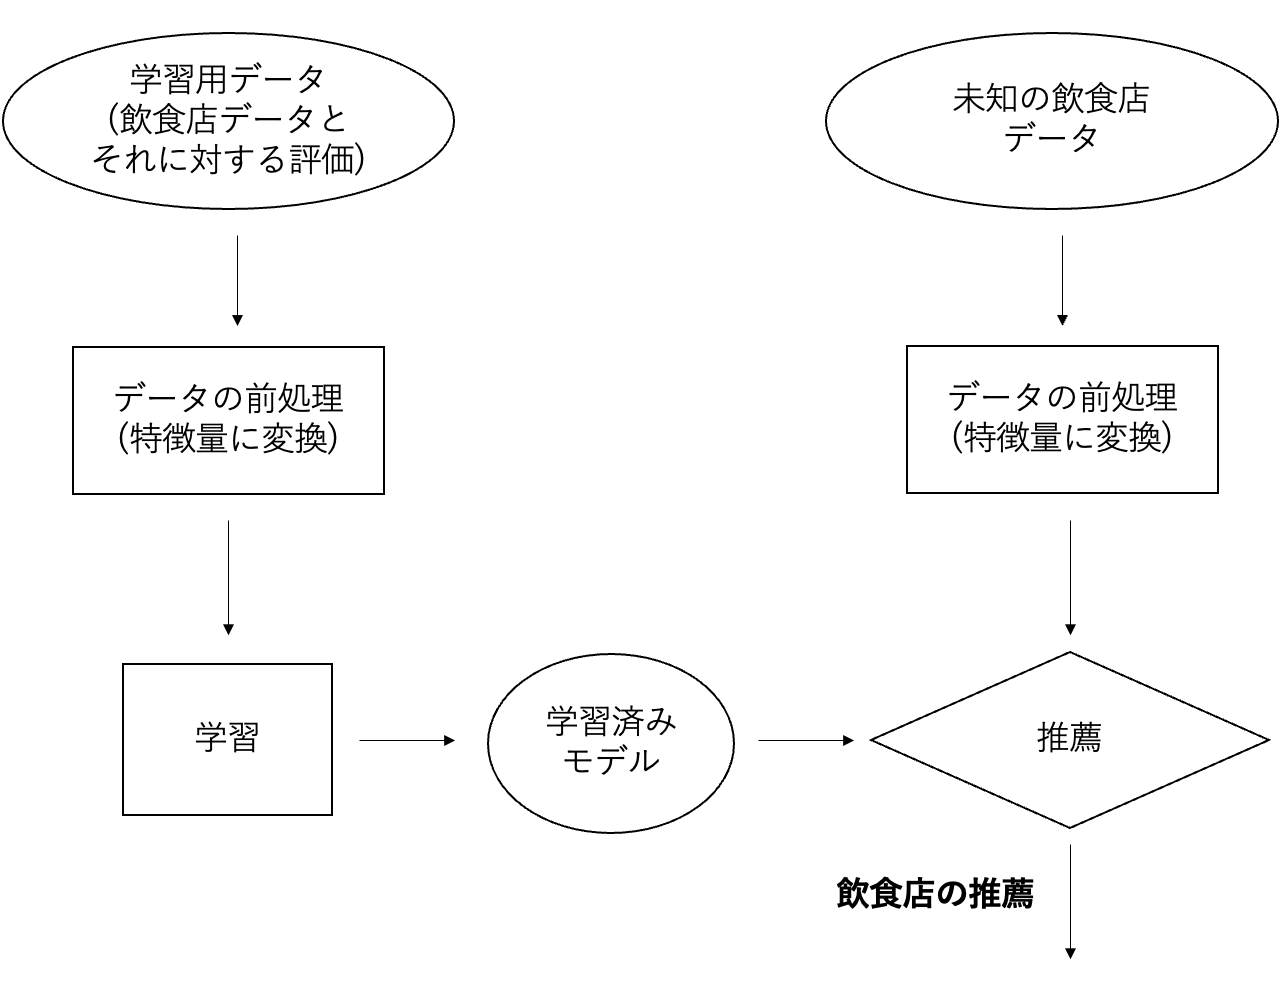
\includegraphics[width=13cm]{image/fig1.png}
    \caption{機械学習を用いた飲食店推薦手法}
    \label{fig1}
  \end{center}
\end{figure}

\section{推薦に用いる飲食店データと特徴量}
本研究で扱う推薦に用いる飲食店データと特徴量は,表\ref{tab:feature_values}の通りで,ジャンル13種類の内訳は,表\ref{tab:genre}の通りである.
これらは0か1といった離散値,0から1にスケーリングされた連続値に変換される.
なお飲食店データは,ホットペッパーグルメとぐるなびから収集したものである.\\\\

\begin{table}[htbp]
  \begin{center}
    \begin{tabular}{|l|c|c|c|c|}\hline
       & \textbf{飲食店データ} & \textbf{特徴量} \\ \hline
      ジャンル(13種類) & なし,あり & 0, 1のベクトル \\ \hline
      個室の有無 & なし, あり & 0, 1 \\ \hline
      喫煙席の有無 & 禁煙, 一部禁煙, 禁煙不可 & 0, 0.5, 1 \\ \hline
      Wi-Fiの有無 & なし, あり & 0, 1 \\ \hline
      駐車場の有無 & なし, あり & 0, 1 \\ \hline
      価格帯 & 0〜1000, 1001〜2000... & 0から1の連続値 \\ \hline
      総合評価 & 1から5の小数点以下2桁 & 0から1の連続値 \\ \hline
    \end{tabular}
  \end{center}
  \caption{飲食店データとその特徴量}
  \label{tab:feature_values}
\end{table}

\begin{table}[htbp]
  \begin{center}
    \begin{tabular}{|c|}\hline
      \textbf{ジャンル} \\ \hline
      中華 \\ \hline
      居酒屋  \\ \hline
      和食 \\ \hline
      お好み焼き・もんじゃ \\ \hline
      韓国料理  \\ \hline
      イタリアン・フレンチ \\ \hline
      焼肉・ホルモン  \\ \hline
      洋食 \\ \hline
      アジア・エスニック料理 \\ \hline
      創作料理 \\ \hline
      各国料理 \\ \hline
      ラーメン \\ \hline
    \end{tabular}
  \end{center}
  \caption{ジャンルの内訳}
  \label{tab:genre}
\end{table}

\section{比較するアルゴリズム\cite{e}}

\subsection{決定木}
決定木とは,木構造を用いて条件分岐を繰り返し,分類や回帰を行う機械学習の手法である.
本研究では,目的変数が0(行きたくない),1(行きたい)といった離散値を取るため,分類を用いる.

決定木では,以下のようなノード\( t \)におけるエントロピー\( I(t) \)を考える.\\
\[
I(t) = - \sum_{i=1}^{c} \frac{n_{ti}}{N_t} \log_2 \frac{n_{ti}}{N_t}
\]\\
\( c \)は目的変数のクラス数,
\( N_t \)はノード\( t \)における訓練データのサンプル数,
\( n_{ti} \)はノード\( t \)におけるクラス\( i \)に属する訓練データの数である.
本研究では,0(行きたくない),1(行きたい)の2クラスの分類を用いるため,\( c = 2\)となる.

ここから,図\ref{fig2}のような木構造を構築していく.
エントロピーを使って,以下のように,条件\( h \)でノード\( O \)から子ノード\( {P_1}^h \),\( {P_2}^h \)に分岐させた時の利得\( \Delta I(O→\{{P_1}^h,{P_2}^h\}) \)を計算する.\\
\[
  \Delta I(O→\{{P_1}^h,{P_2}^h\}) = I(O) - \sum_{i=1}^{b} \frac{N_{{P_i}^h}}{N_O} I({P_i}^h)
\]\\
\( b \)は分岐の数である.
本研究では図\ref{fig2}のような,各条件に対する真偽値によって分岐していく2分木を用いるため,\( b = 2\)となる.

このような利得が最大になるような条件を探し,分岐を繰り返す.
なお,本研究では,全ての葉ノードで,片方のクラスのデータのみが格納されるまで分岐を繰り返す.
そして,得られた木構造を元に,属するクラスを予測する.

表\ref{table}のような飲食店A,B,C,D,Eの特徴量と,それらに対するユーザーの評価値を使って,飲食店Fを推薦するかどうかを考える.
まず,ルートノード\(O\)には飲食店A,B,C,D,Eの特徴量とそれらに対するユーザーの評価値が含まれるため,初期のエントロピー\(I(O)\)は以下の通りである.\\
\[
I(O) = - \frac{2}{5} \log_2 \frac{2}{5} - \frac{3}{5} \log_2 \frac{3}{5} = 0.97
\]\\
次に,どのような条件で子ノード\(P_1,P_2\)に分岐させると,利得が高いのかを求める.
駐車場の有無\(p\)を条件とし,子ノード\({P_1}^p,{P_2}^p\)に分岐させた場合は以下の通りである.\\

\begin{align*}
  \Delta I(O→\{{P_1}^p,{P_2}^p\}) 
  &= I(O) - \sum_{i=1}^{2} \frac{N_{{P_i}^p}}{N_O} I({P_i}^p)\\ 
  &= 0.97 - \{\frac{1}{5} (- \frac{1}{1} \log_2 \frac{1}{1} - \frac{0}{0} \log_2 \frac{0}{0}) + \frac{4}{5} (- \frac{2}{4} \log_2 \frac{2}{4} - \frac{2}{4} \log_2 \frac{2}{4})\}\\
  &= 0.17
\end{align*}
個室の有無\(r\)を条件とし,子ノード\({P_1}^r,{P_2}^r\)に分岐させた場合は以下の通りである.\\

\begin{align*}
  \Delta I(O→\{{P_1}^r,{P_2}^r\}) 
  &= I(O) - \sum_{i=1}^{2} \frac{N_{{P_i}^r}}{N_O} I({P_i}^r)\\ 
  &= 0.97 - \{\frac{2}{5} (- \frac{1}{2} \log_2 \frac{1}{2} - \frac{1}{2} \log_2 \frac{1}{2}) + \frac{3}{5} (- \frac{2}{3} \log_2 \frac{2}{3} - \frac{1}{3} \log_2 \frac{1}{3})\}\\
  &= 0.02
\end{align*}\\
喫煙席の有無\(s\)を条件とし,子ノード\({P_1}^s,{P_2}^s\)に分岐させた場合は以下の通りである.\\

\begin{align*}
  \Delta I(O→\{{P_1}^s,{P_2}^s\}) 
  &= I(O) - \sum_{i=1}^{2} \frac{N_{{P_i}^s}}{N_O} I({P_i}^s)\\ 
  &= 0.97 - \{\frac{3}{5} (- \frac{1}{3} \log_2 \frac{1}{3} - \frac{2}{3} \log_2 \frac{2}{3}) + \frac{2}{5} (- \frac{2}{2} \log_2 \frac{2}{2} - \frac{0}{0} \log_2 \frac{0}{0})\}\\
  &= 0.42
\end{align*}\\

結果として,ルートノード\(O\)から子ノード\(P\)に分岐させる条件は,「喫煙席の有無」であった.
「喫煙席の有無」という条件で分岐させると,ノード\(P_1\)は片方のクラスのデータのみが格納されている状態になり,これ以上分岐できない.

ノード\(P_2\)のエントロピー\(I(P_2)\)は以下の通りである.\\
\[
I(P_2) = - \frac{1}{3} \log_2 \frac{1}{3} - \frac{2}{3} \log_2 \frac{2}{3} = 0.92
\]\\
次に,「喫煙席の有無」以外で,どのような条件で子ノード\(R_1,R_2\)に分岐させると利得が高いのかを求める.
駐車場の有無\(p\)を条件とし,子ノード\({R_1}^p,{R_2}^p\)に分岐させた場合は以下の通りである.\\
\begin{align*}
  \Delta I(P_2→\{{R_1}^p,{R_2}^p\})
  &= I(P_2) - \sum_{i=1}^{2} \frac{N_{{R_i}^p}}{N_{P_2}} I({R_i}^p)\\ 
  &= 0.92 - \{\frac{1}{3} (- \frac{1}{1} \log_2 \frac{1}{1} - \frac{0}{0} \log_2 \frac{0}{0}) + \frac{2}{3} (- \frac{0}{0} \log_2 \frac{0}{0} - \frac{2}{2} \log_2 \frac{2}{2})\}\\
  &= 0.92
\end{align*}\\
個室の有無\(r\)を条件とし,子ノード\({R_1}^r,{R_2}^r\)に分岐させた場合は以下の通りである.\\
\begin{align*}
  \Delta I(P_2→\{{R_1}^r,{R_2}^r\})
  &= I(P_2) - \sum_{i=1}^{2} \frac{N_{{R_i}^r}}{N_{P_2}} I({R_i}^r)\\ 
  &= 0.92 - \{\frac{1}{3} (- \frac{0}{0} \log_2 \frac{0}{0} - \frac{1}{1} \log_2 \frac{1}{1}) + \frac{2}{3} (- \frac{1}{2} \log_2 \frac{1}{2} - \frac{1}{2} \log_2 \frac{1}{2})\}\\
  &= 0.25
\end{align*}

結果として,ルートノード\(P_2\)から子ノード\(R_1,R_2\)に分岐させる条件は,「駐車場の有無」であった.
「駐車場の有無」という条件で分岐させると,ノード\(R_1\),ノード\(R_2\)は片方のクラスのデータのみが格納されている状態になり,これ以上分岐する必要が無い.
これで全ての葉ノードで片方のクラスのデータのみが格納されている状態になるため,図\ref{fig10}のような決定木が構築される.
飲食店Fは青色のノード\(P_1\)に格納され,飲食店Fに対する予測評価値は0になるため,Fを推薦しない.

機械学習ライブラリであるScikit-LearnのDecisionTreeClassifierクラスを用いて,ソースコード\ref{入力変数と目的変数の設定},\ref{決定木}のように実装している.\\

\begin{figure}[htbp]
  \begin{center}
    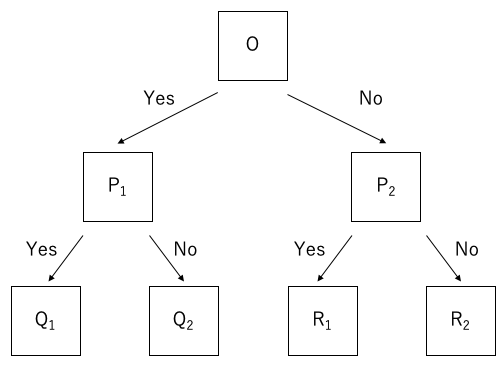
\includegraphics[width=10cm]{image/fig2.png}
    \caption{決定木}
    \label{fig2}
  \end{center}
\end{figure}

\begin{figure}[htbp]
  \begin{center}
    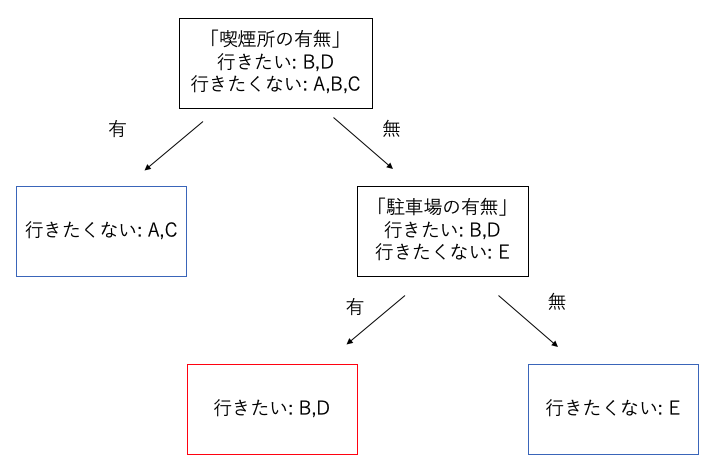
\includegraphics[width=10cm]{image/fig10.png}
    \caption{得られた決定木}
    \label{fig10}
  \end{center}
\end{figure}

\begin{table}[htbp]
  \begin{center}
    \begin{tabular}{|l|r|r|r|r|}\hline
      \textbf{飲食店/特徴} & 駐車場の有無 & 個室の有無 & 喫煙席の有無  &  ユーザーの評価値 \\ \hline
      飲食店A     & 1        & 1        & 1        & 0 \\ \hline
      飲食店B     & 1      & 0        & 0        & 1 \\ \hline
      飲食店C     & 1      & 0        & 1        & 0 \\ \hline
      飲食店D     & 1        & 1        & 0        & 1 \\ \hline
      飲食店E     & 0        & 1        & 0        & 0 \\ \hline
      飲食店F     & 0        & 0        & 1        & - \\ \hline
    \end{tabular}
  \end{center}
  \caption{飲食店の特徴量とそれに対するユーザーの評価の例}
  \label{table}
\end{table}

\begin{lstlisting}[caption=特徴ベクトルと目的変数の設定,label=入力変数と目的変数の設定]
import numpy as np

# 飲食店A, B, C, D, Eの特徴ベクトルの設定
features = np.array([
  [1, 1, 1],  
  [1, 0, 0],  
  [1, 0, 1],  
  [1, 1, 0],  
  [0, 1, 0]   
])

# 目的変数の設定
labels = np.array([0, 1, 0, 1, 0])

# 飲食店Fの特徴ベクトルの設定
feature_F = np.array([[0, 0, 1]])
\end{lstlisting}

\begin{lstlisting}[caption=決定木による予測,label=決定木]
from sklearn.tree import DecisionTreeClassifier

# 決定木モデルをインスタンス化
dtc = DecisionTreeClassifier()

# 決定木モデルの訓練
dtc.fit(features, labels)

# 飲食店Fに対する予測
prediction_F = dtc.predict(feature_F)

# 出力:0
print(prediction_F)
\end{lstlisting}

\subsection{ロジスティック回帰}
ロジスティック回帰とは,線形モデルの1つであり,陽性クラス(本研究では「行きたい」のクラス)に属する確率を用いて,2クラス分類を行う機械学習の手法である.
本研究では,目的変数が0(行きたくない),1(行きたい)の2クラスを取るため,この手法を用いることができる.

ロジスティック回帰では,以下のようなシグモイド関数\( \sigma(t) \)を考える.\\
\[
\sigma(t) = \frac{1}{1 + e^{-t}}
\]\\

シグモイド関数\( \sigma(t) \)に,\( t = \sum_{i=0}^{n} w_i x_i \)を代入し,未知のデータが陽性クラスに属する確率\( \hat{p} \)を求める.\\
\[
\hat{p} = \sigma\left(\sum_{i=0}^{n} w_i x_i\right)
\]\\
\( n \)は特徴量の数,\( x_i \)は\( i \)番目の特徴量,\( w_i \)は\( i \)番目の特徴量に対する重みである.
本研究では,特徴量の数は,表\ref{tab:feature_values}と表\ref{tab:genre}で示した通りで,19なので,\( n = 19 \)となる.
下記のような損失関数\( E \)を考える.\\
\[
E = - \frac{1}{m} \sum_{j=1}^{m} \left[ y_j \log(\hat{p}_j) + (1 - y_j) \log(1 - \hat{p}_j) \right]
\]\\
\( m \)は訓練データの数,\( y_j \)は\( j \)番目のデータに対する目的変数,\( \hat{p}_j \)は\( j \)番目のデータが陽性クラスに属する確率である.
損失関数\( E \)を用いた勾配降下法で,最適な\( w_i(0 \leq i \leq n) \)を見つける.
重み\( w_i  = 0 (0 \leq i \leq n) \)から開始し,収束するまで下記のような勾配降下を行う.\\
\[
  w_i ← w_i - \frac{\partial E}{\partial w_i} ・ \alpha
\]\\
\( \alpha \)は学習率である.
そして,予測モデル\( \hat{y} \)は,以下のように定式化される.\\
\[
\hat{y} = 
\begin{cases} 
0 & \text{if } \hat{p} \leq 0.5 \\
1 & \text{if } \hat{p} > 0.5 
\end{cases}
\]\\
この予測モデルは,陽性クラスに属する確率が0.5以下であれば,陰性クラスと予測し,陽性クラスに属する確率が0.5を超えていれば,陽性クラスと予測することを示している.

表\ref{table}のような飲食店A,B,C,D,Eの特徴量と,それらに対するユーザーの評価値を使って,飲食店Fを推薦するかどうかを考える.
ここで,駐車場の有無を\( x_1 \),個室の有無を\( x_2 \),喫煙席の有無を\( x_3 \)とする.
また,それらに対する重みをそれぞれ\( w_1 = 0 \),\( w_2 = 0 \),\( w_3 = 0 \)から開始する.
損失関数\( E \)は以下のように定義される.\\

\begin{align*}
E &= - \frac{1}{5} \sum_{j=1}^{5} \left[ y_j \log(\hat{p}_j) + (1 - y_j) \log(1 - \hat{p}_j) \right]\\
&= - \frac{1}{5} ( \log(1 - \hat{p}_1) + \log(\hat{p}_2) + \log(1 - \hat{p}_3) + \log(\hat{p}_4) + \log(1 - \hat{p}_5))\\
&= - \frac{1}{5} \{ \log(1 - \sigma(w_1 + w_2 + w_3)) + \log(\sigma(w_1)) + \log(1 - \sigma(w_1 + w_3)) \\
&+ \log(\sigma(w_1 + w_2)) + \log(1 - \sigma(w_2))\}
\end{align*}\\
損失関数\( E \)を用いて,学習率\( \alpha = 0.01\)で勾配降下を1度行うと,\( w_1 = 0 \),\( w_2 = -0.001 \),\( w_3 = -0.002 \)となった.
これを繰り返すと,\( w_1 = 0 \),\( w_2 = -0.219 \),\( w_3 = -0.690 \)と収束した.
飲食店Fが陽性クラスに属する確率\(\hat{p_f}\)は以下の通りである.\\
\begin{align*}
  \hat{p_f} &= \sigma\left( 0 * 0 + (-0.219) * 0 + (-0.690) * 1\right) \\
  &= 0.334
\end{align*}\\
飲食店Fが陽性クラスに属する確率は0.5以下であるため,飲食店Fを推薦しない.

機械学習ライブラリであるScikit-LearnのLogisticRegressionクラスを用いて,ソースコード\ref{入力変数と目的変数の設定},\ref{ロジスティック回帰}のように実装している.\\

\begin{lstlisting}[caption=ロジスティック回帰による予測,label=ロジスティック回帰]
from sklearn.linear_model import LogisticRegression

# ロジスティック回帰モデルをインスタンス化
lr = LogisticRegression()

# ロジスティック回帰モデルの訓練
lr.fit(features, labels)

# 飲食店Fに対する予測
prediction_F = lr.predict(feature_F)

# 出力:0
print(prediction_F)
\end{lstlisting}

\subsection{k-NN}
k-NNとは,非線形モデルの1つで,近傍データ\( k \)個で多数決を行い,クラス分類を行う機械学習の手法である.
本研究では,目的変数が0(行きたくない),1(行きたい)の2クラスを取るため,この手法を用いることができる.

本研究では,訓練データの特徴ベクトル\( x \)と予測対象のデータの特徴ベクトル\( y \)の距離を考える.
計算に以下のようなユークリッド距離\( d(x, y) \)を用いる.\\\\
\[
d(x, y) = \sqrt{\sum_{i=1}^{n} (x_i - y_i)^2}
\]\\\\
\( n \)は特徴量の数,\( x_i \)は訓練データの\( i \)番目の特徴量,\( y_i \)は,予測対象であるデータの\( i \)番目の特徴量.
本研究では,特徴量の数は,表\ref{tab:feature_values}と表\ref{tab:genre}で示した通りで,19なので,\( n = 19 \)となる.
つまり,最も予測対象のデータ\( y \)と近い訓練データ\( x \)を\( k \)個見つけ,その\( k \)個の目的変数の多数決によって,属するクラスを予測するのである.

表\ref{table}のような飲食店A,B,C,D,Eの特徴量と,それらに対するユーザーの評価値を使って,飲食店Fを推薦するかどうかを考える.
ここで,飲食店Fの\( i \)番目の特徴量を\( y_i \),その他の飲食店の\( i \)番目の特徴量を\( x_i \),\( k = 3 \)とする.
図\ref{fig3}のように,飲食店Fと飲食店Aのユークリッド距離は1.41,飲食店Fと飲食店Bのユークリッド距離は1.41,飲食店Fと飲食店Cのユークリッド距離は1.0,飲食店Fと飲食店Dのユークリッド距離は1.73,飲食店Fと飲食店Eのユークリッド距離は1.41となる.
つまり,近傍データ3つは,飲食店A,B,C(データセット内で最初に出現するデータを選択するため,飲食店Eは除外)となり,これら3つの目的変数で多数決をしても0になるため,飲食店Fに対する予測評価値は0になるため,飲食店Fを推薦しない.

機械学習ライブラリであるScikit-LearnのKNeighborsClassifierを用いて,ソースコード\ref{入力変数と目的変数の設定},\ref{k-NN}のように実装している.
また,GridSearchCVを用いて,\( k \)の範囲を指定し,範囲内の\( k \)の中から,交差検証で最も精度が良かった時の値に設定する.\\

\begin{lstlisting}[caption=k-NNによる予測,label=k-NN]
from sklearn.neighbors import KNeighborsClassifier
from sklearn.model_selection import GridSearchCV

# kを1から5に設定
param_grid = {'n_neighbors': range(1, 5)}

# k-NNモデルをインスタンス化
knn = KNeighborsClassifier()

# k=1から5における5つのモデルで, 5フォールド交差検証を行うための, 5つのモデルが格納されたクラスのインスタンス化
grid_search = GridSearchCV(knn, param_grid, cv=5, scoring='precision')

# GridSearchモデルの訓練
grid_search.fit(features, labels)

# 最も精度が良かったモデルを取り出す
best_knn = grid_search.best_estimator_

# 最も精度が良かったモデルで飲食店Fに対する予測
prediction_F = best_knn.predict(feature_F)

# 出力:0
print(prediction_F) 
\end{lstlisting}

\vspace{5mm}

\begin{figure}[htbp]
  \begin{center}
    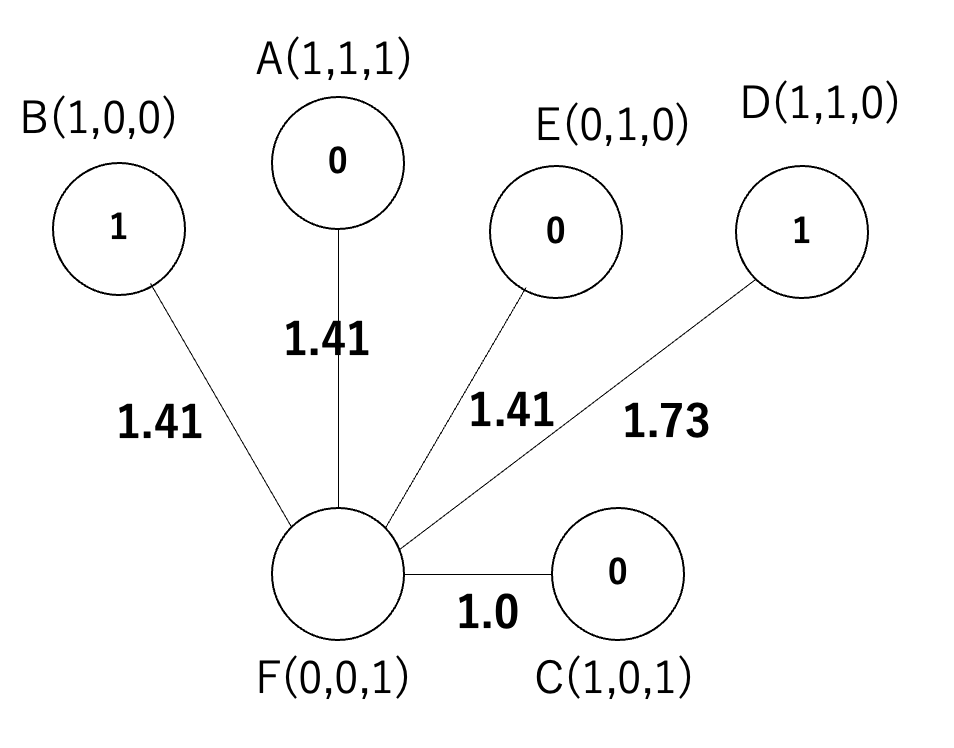
\includegraphics[width=12cm]{image/fig3.png}
    \caption{飲食店Fとその他の飲食店の距離}
    \label{fig3}
  \end{center}
\end{figure}

% 4章

\chapter{評価}
\section{評価の目的}
飲食店推薦に,決定木,ロジスティック回帰,k-NNのうち,どの機械学習アルゴリズムを用いることが有用であるかどうかを調べる.

\section{評価方法}
以下の手順で,決定木,ロジスティック回帰,k-NNの比較を行う.\\

・実験協力者3人に,ホットペッパーグルメとぐるなびから取得した飲食店データ100件分を見せ,「行きたい」「行きたくない」といった評価を取得する.\\

・飲食店データを変換した特徴ベクトルと,飲食店に対する評価を数値(「行きたくない」を0,「行きたい」を1)に変換した目的変数を1個のデータセットとし,1人あたり100個のデータセットを作成する.\\

・各手法の10フォールド交差検証を行い,精度と再現率を算出する.
なお,10フォールド交差検証は,データセット100個のうち,訓練データ90個,テストデータ10個の検証を,異なる組み合わせで10通り行うことである.\\

・10フォールド交差検証で得られた各手法の精度間に統計的な有意差があるかどうかをウィルコクソンの符号順位検を用いて確認する.\\

また,それぞれのアルゴリズムで,訓練データの数を10から90に増やした際に,精度がどのように推移するかどうかも確かめる.
本研究では,決定木,ロジスティック回帰,k-NNの性能を,以下のような評価指標を用いて評価する.\\\\
\textbf{精度}\\
「行きたい」と予測したもののうち,「行きたい」ものの割合.\\\\\\
\textbf{再現率}\\
「行きたい」もののうち,「行きたい」と予測したものの割合.\\

また,最も良かった手法と他の手法の精度に有意差があるかどうかを,以下の検定を用いて確認する.\\\\
\textbf{ウィルコクソンの符号順位検定}\\
最も平均精度が良かったアルゴリズムで得られた10個の精度と,その他のアルゴリズムで得られた10個の精度を用いて,以下の手順で検定を行う.\\\\
・2群間における各ペアについて差を計算する.\\\\
・各ペアの差の絶対値を取り,これらを小さい順に順位付けする.\\\\
・各差に正または負の符号(元の差が正の場合は正,負の場合は負)を付ける.\\\\
・正の順位の合計と負の順位の合計をそれぞれ計算する.\\\\
・正の順位の合計と負の順位の合計のうち,小さい方の合計が検定統計量とする.\\\\
・ウィルコクソンの符号順位検定の分布表を参照し,サンプルサイズと検定統計量に対応するp値が求められる.\\\\
・p値が0.05以下であれば,2群間に統計的な有意差があると結論付ける.

\section{結果}
\subsection{10フォールド交差検証で得られた結果}
各アルゴリズムで10フォールド交差検証を行ったところ,精度は図\ref{fig7},再現率は図\ref{fig8}のようになった.
精度,再現率ともに決定木が最も良かった.
また,最も精度が良かった決定木と他のアルゴリズムの精度間に,統計的な有意差が存在するかどうかを調べるために,10フォールド交差検証の精度を使ってウィルコクソンの符号順位検を行った.
ランダム手法と決定木の間では,ユーザー3人において,有意水準1%で有意差が見られた.
なお,ランダム手法はテストデータを全て「行きたい」と予測する手法である.
ロジスティック回帰と決定木の間ではユーザー1,ユーザー2において,有意水準5%で有意差が見られた.
k-NNと決定木の間では,ユーザー2,ユーザーにおいて,有意水準5%で有意差が見られた.

\begin{figure}[htbp]
  \begin{center}
    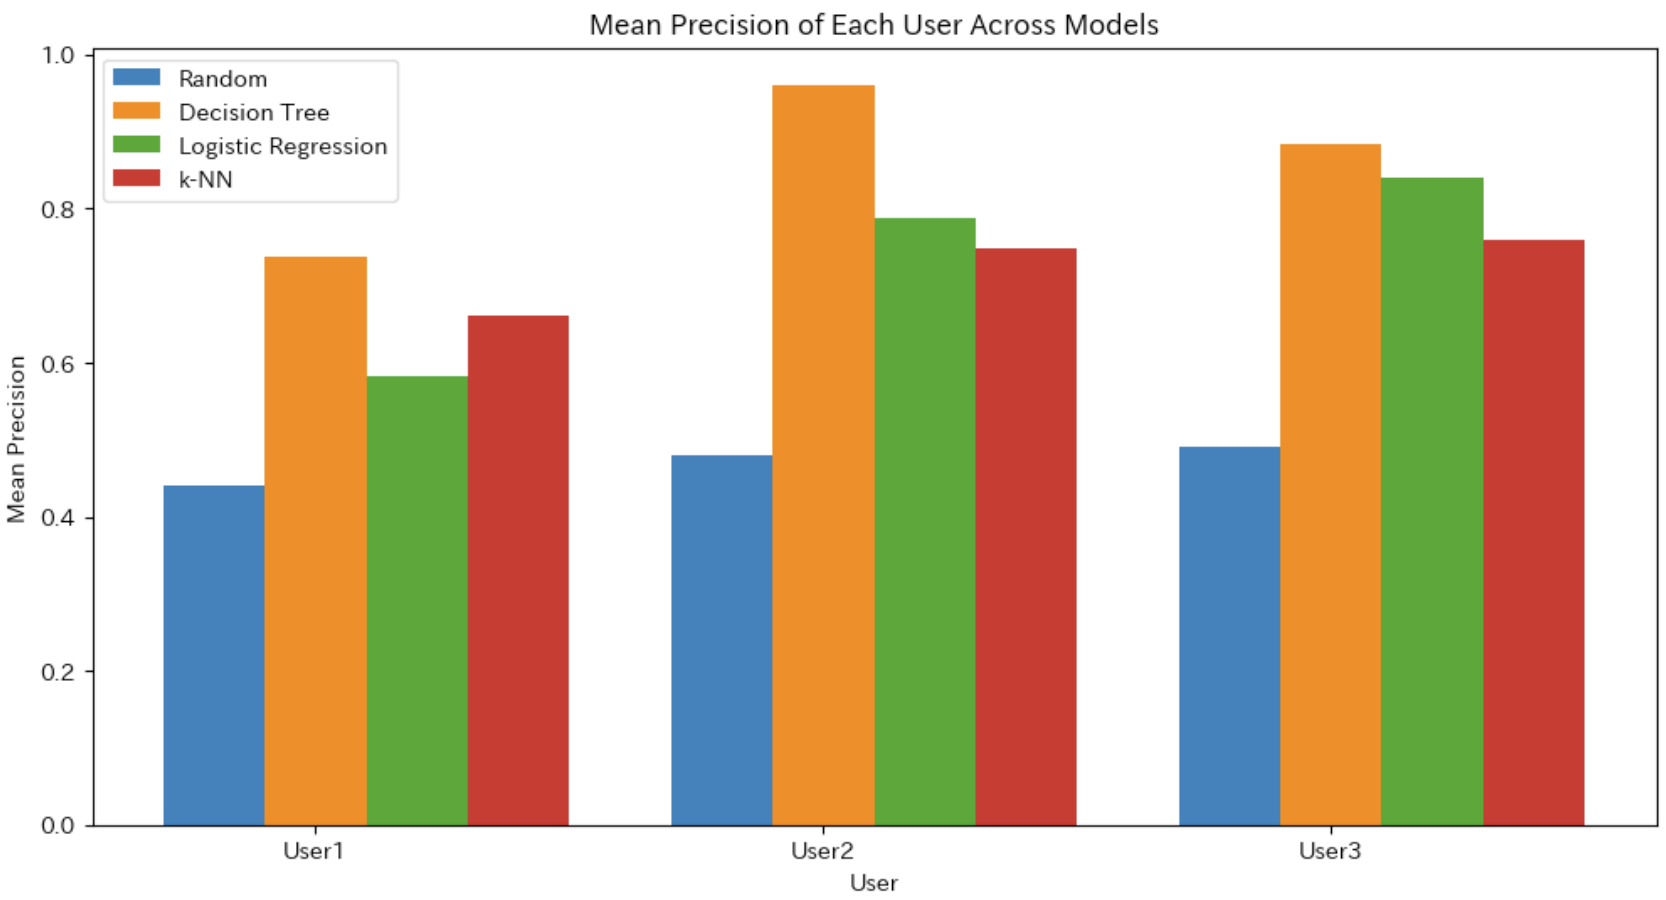
\includegraphics[width=14cm]{image/fig7.png}
    \caption{10フォールド交差検証で得られた精度}
    \label{fig7}
  \end{center}
\end{figure}

\begin{figure}[htbp]
  \begin{center}
    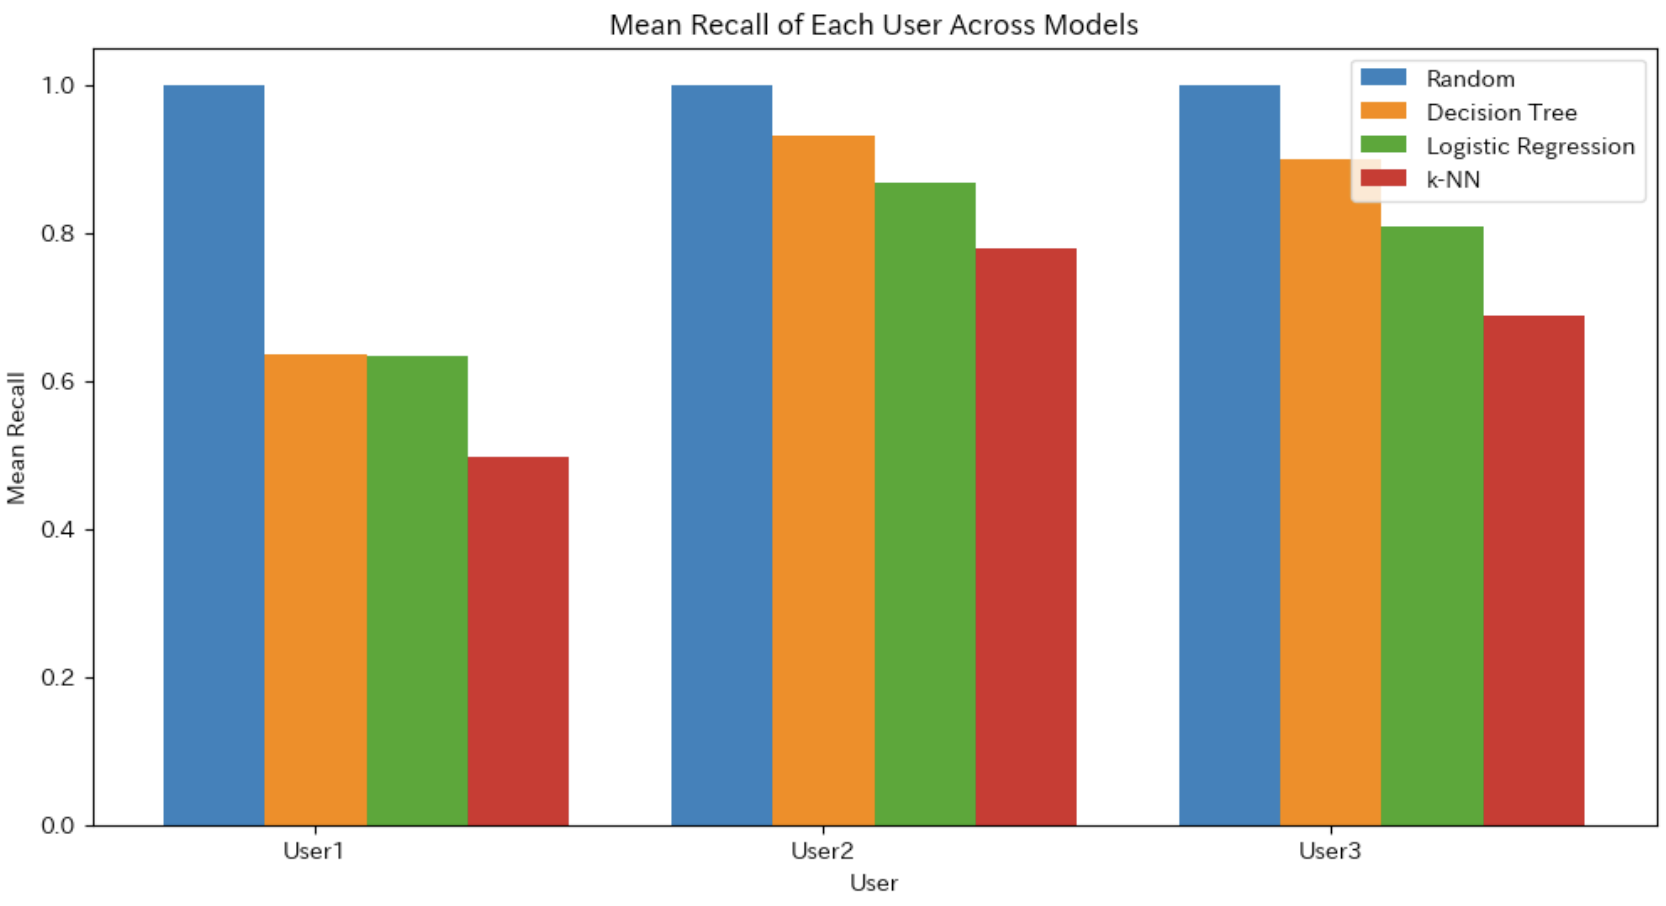
\includegraphics[width=14cm]{image/fig8.png}
    \caption{10フォールド交差検証で得られた再現率}
    \label{fig8}
  \end{center}
\end{figure}

\begin{table}[htbp]
  \begin{center}
    \begin{tabular}{|l|r|r|r|r|}\hline
      \textbf{手法/ユーザー} & ユーザー1 & ユーザー2 & ユーザー3 \\ \hline
      ランダム手法       & ○        & ○        & ○  \\ \hline
      ロジスティック回帰       & ○        & ○        & × \\ \hline
      k-NN       & ×       & ○        & ○       \\ \hline
    \end{tabular}
  \end{center}
  \caption{決定木と他手法の精度における統計的な有意差}
  \label{Significant_difference_table}
\end{table}

\begin{figure}[htbp]
  \begin{center}
    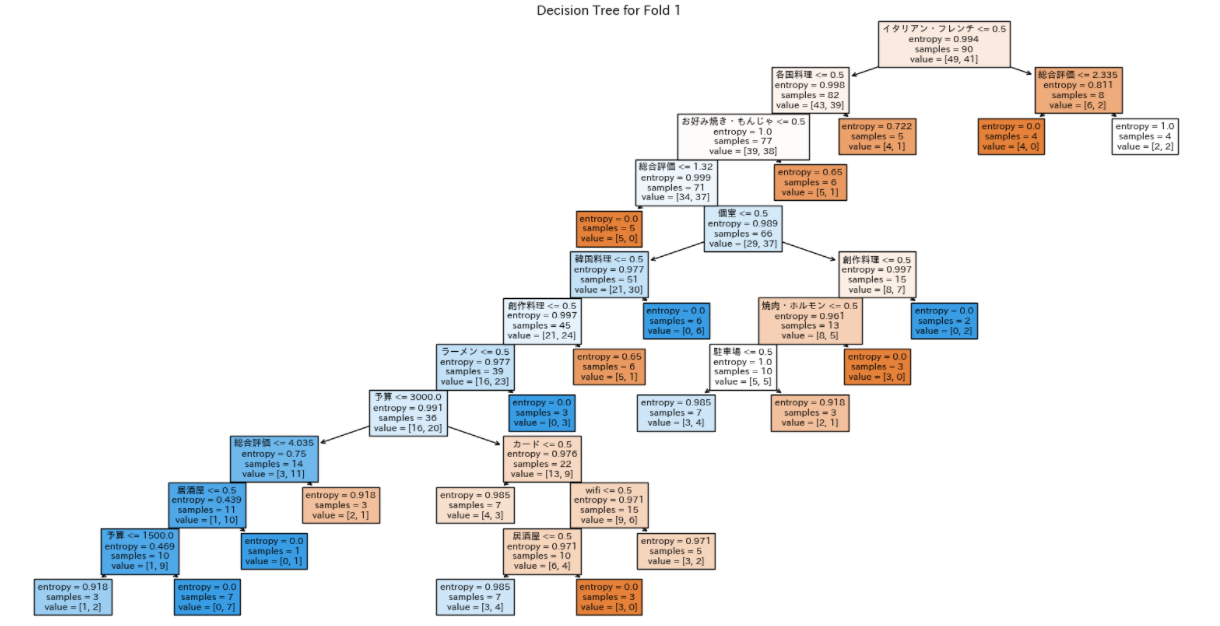
\includegraphics[width=14cm]{image/fig4.png}
    \caption{ユーザー1の決定木}
    \label{fig4}
  \end{center}
\end{figure}

\begin{figure}[htbp]
  \begin{center}
    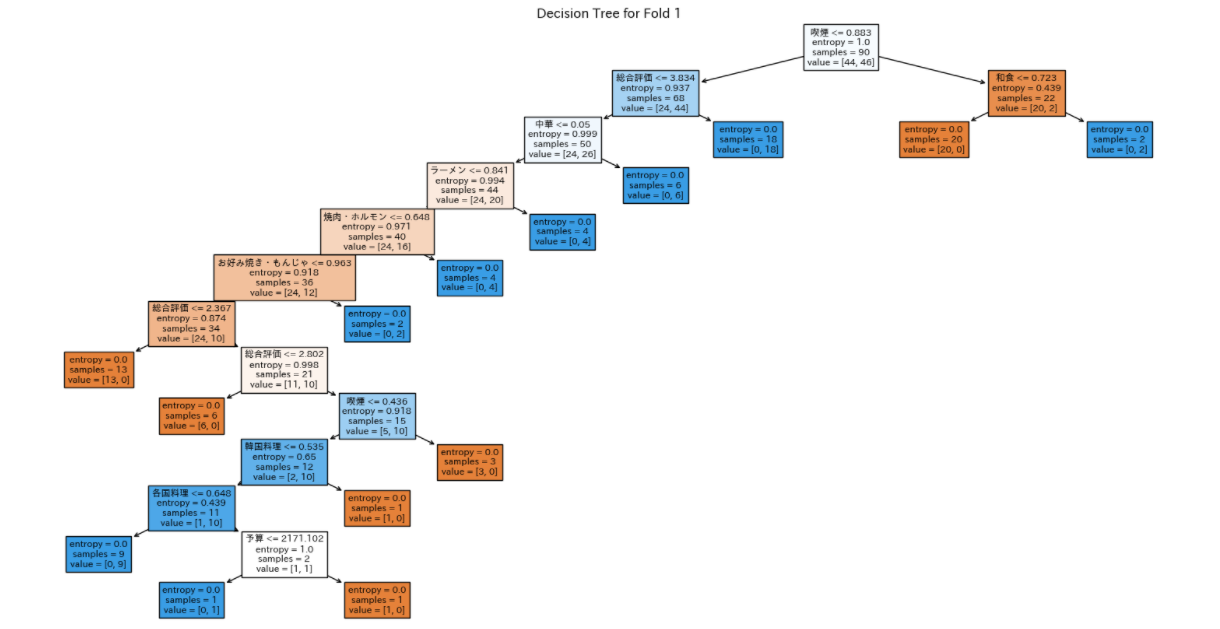
\includegraphics[width=14cm]{image/fig5.png}
    \caption{ユーザー2の決定木}
    \label{fig5}
  \end{center}
\end{figure}

\begin{figure}[htbp]
  \begin{center}
    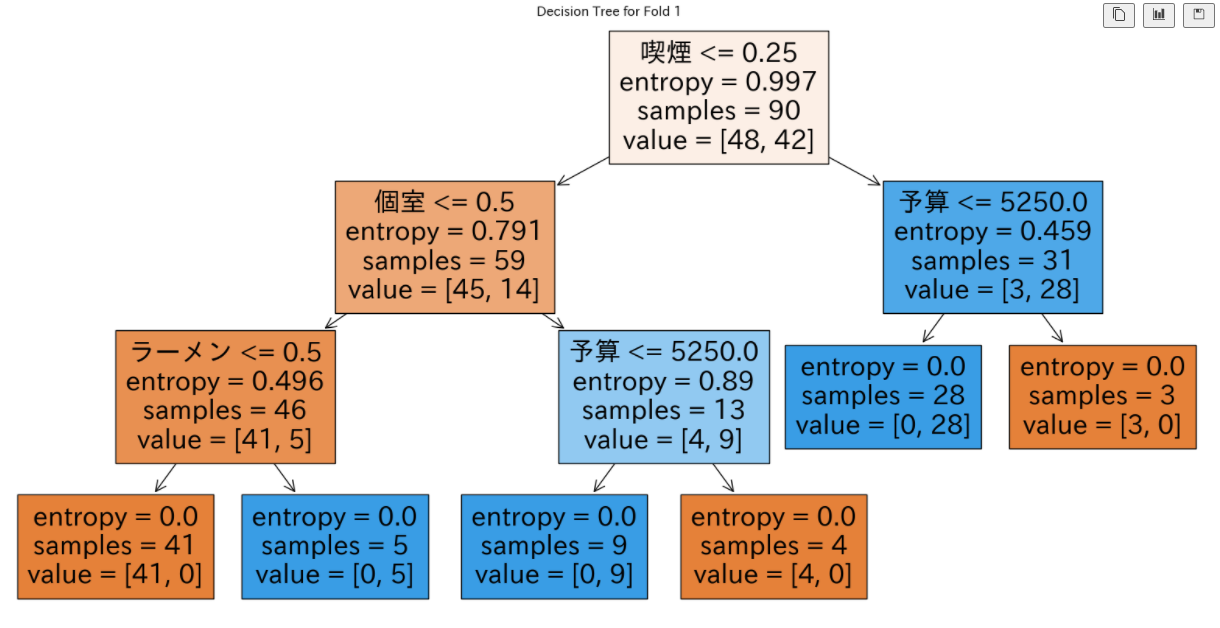
\includegraphics[width=12cm]{image/fig6.png}
    \caption{ユーザー3の決定木}
    \label{fig6}
  \end{center}
\end{figure}

\subsection{訓練データを増やした際の精度の推移}
各アルゴリズムにおいて,訓練データを増やした際の精度の推移を図\ref{fig9}に示している.
訓練データが少ない状況では,ロジスティック回帰が最も良い精度を示し,逆に訓練データが多い状況では,決定木が最も良い精度を示した.\\

\begin{figure}[htbp]
  \begin{center}
    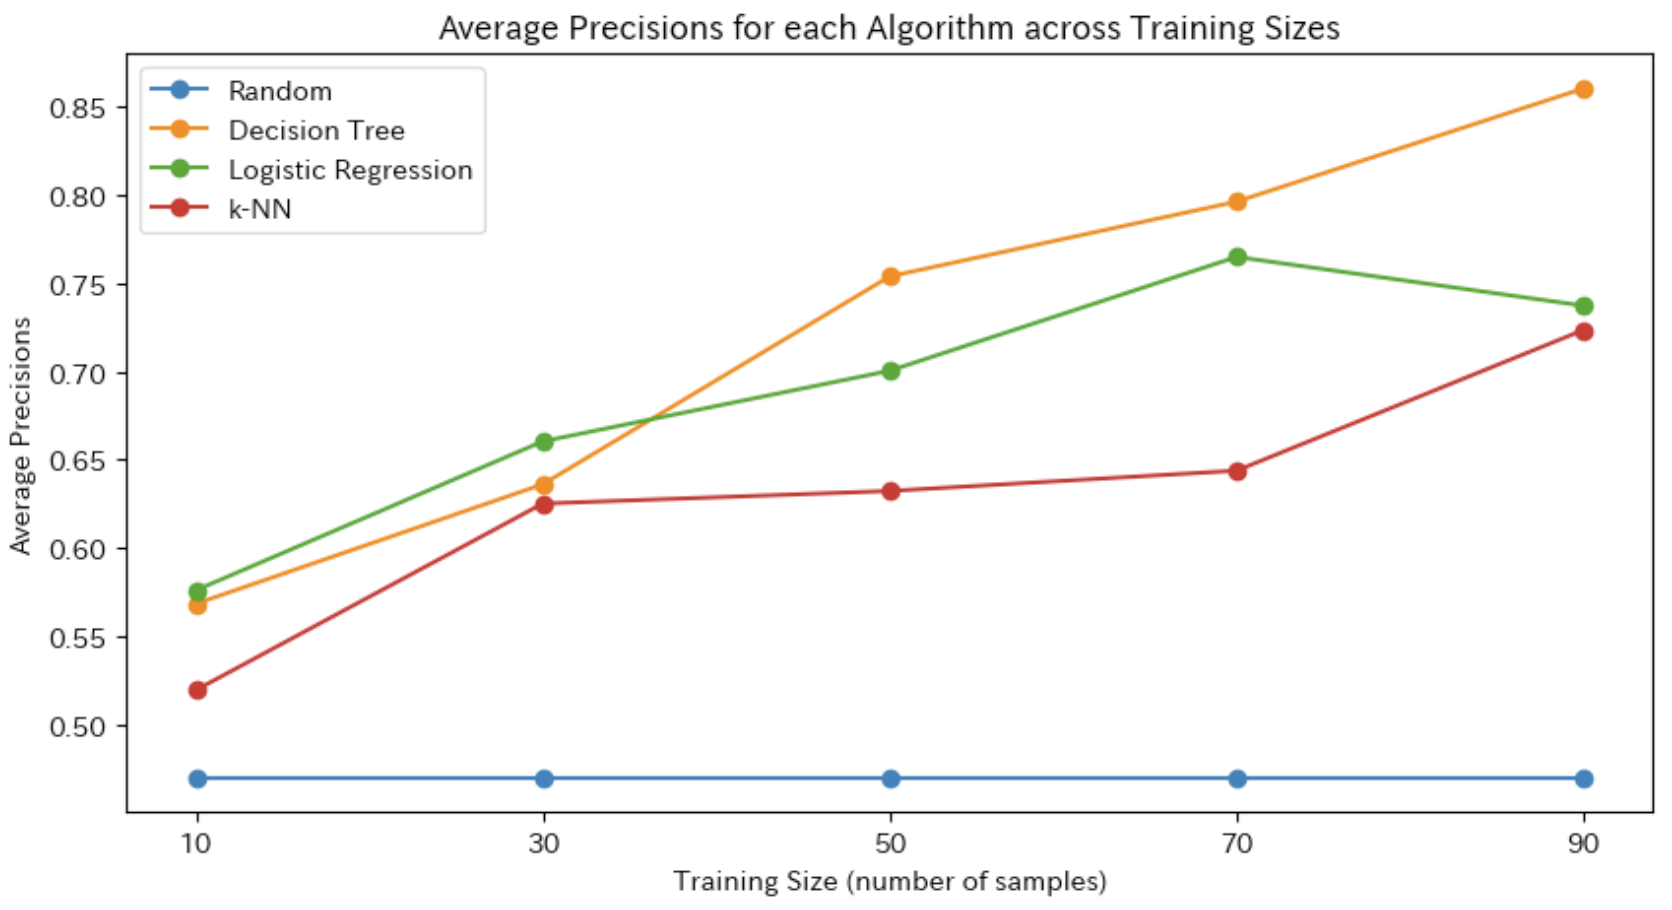
\includegraphics[width=14cm]{image/fig9.png}
    \caption{訓練データを増やした際の精度の推移}
    \label{fig9}
  \end{center}
\end{figure}

\subsection{結果の考察}
図\ref{fig7}を見ると,ユーザー1とユーザー2に比べて,ユーザー3の決定木と他の手法の精度の差が小さいことが分かる.
また,図\ref{fig4},図\ref{fig5},図\ref{fig6}を見ると,ユーザー1とユーザー2に比べて,ユーザー3は簡単な決定木が作成されていることが分かる.
つまり,簡単な決定木が作られたユーザーに対しては,決定木と他の手法の精度の差が小さいと言える.
逆に,複雑な決定木が作られたユーザーに対しては,決定木と他の手法の精度の差が大きいため,より決定木の有効性が増すと言える.

図\ref{fig9}を見ると,訓練データが少ない状況では,ロジスティック回帰が最も良い精度を示しているが,3つの手法はランダム手法とあまり変わらない精度であった.
訓練データが50になったところで,決定木が最も良い精度を示しており,訓練データが90の時も決定木が最も良い精度を示している.
つまり,ユーザーの評価データが十分に集まらない環境であれば,飲食店推薦にはロジスティック回帰を応用するのが最も良いと言える.
逆に,ユーザーの評価データが十分に集まる環境であれば, 飲食店推薦には決定木を応用するのが最も良いと言える.

\chapter{まとめ}

本研究は,内容ベースフィルタリングを用いた飲食店推薦において,決定木,ロジスティック回帰,k-NNのうち,どの機械学習アルゴリズムを使えばいいかを明確化することを目的として行われた.
その結果,内容ベースフィルタリングを用いた飲食店推薦には,ユーザーの評価データが十分に集まる環境であれば, 決定木を応用することが適していることが分かった.

今後の課題は,写真や口コミ,位置情報といった,他にも考慮すべき特徴が存在するため,そのような特徴も考慮できるようにすることである.

\appendix

\acknowledgement %謝辞

本研究を進めるにあたり,終始ご指導下さった北村泰彦教授に深く感謝いたします.

また,飲食店の評価に協力して頂いた友人3名にお礼申し上げます.

北村研究室の同輩諸氏には,日頃から多くのご助言やご支援をいただき,大変感謝しています.

最後に,4年間大学に通わせてくれた両親に,心から感謝しています.

\reference{sample} %bibファイル名を指定

\end{document}
